\documentclass[12pt]{article}
\usepackage{geometry}
\usepackage{fullpage}
\usepackage{graphicx}
\geometry{a4paper}
\setlength\parindent{0pt}
\title{Deliverable 6}
\author{
    Gordon Reid: 1002536R\\
    Ryan Wells: 1002253W\\
    Kristopher Stewart: 1007175S\\
    David Selkirk: 1003646S\\
    James Gallagher: 0800899G\\
}
\date{\today}

\begin{document}

\maketitle

\newpage

\tableofcontents

\newpage

\section{Introduction}

\newpage

\section{System Architecture}

\subsection{Diagram}

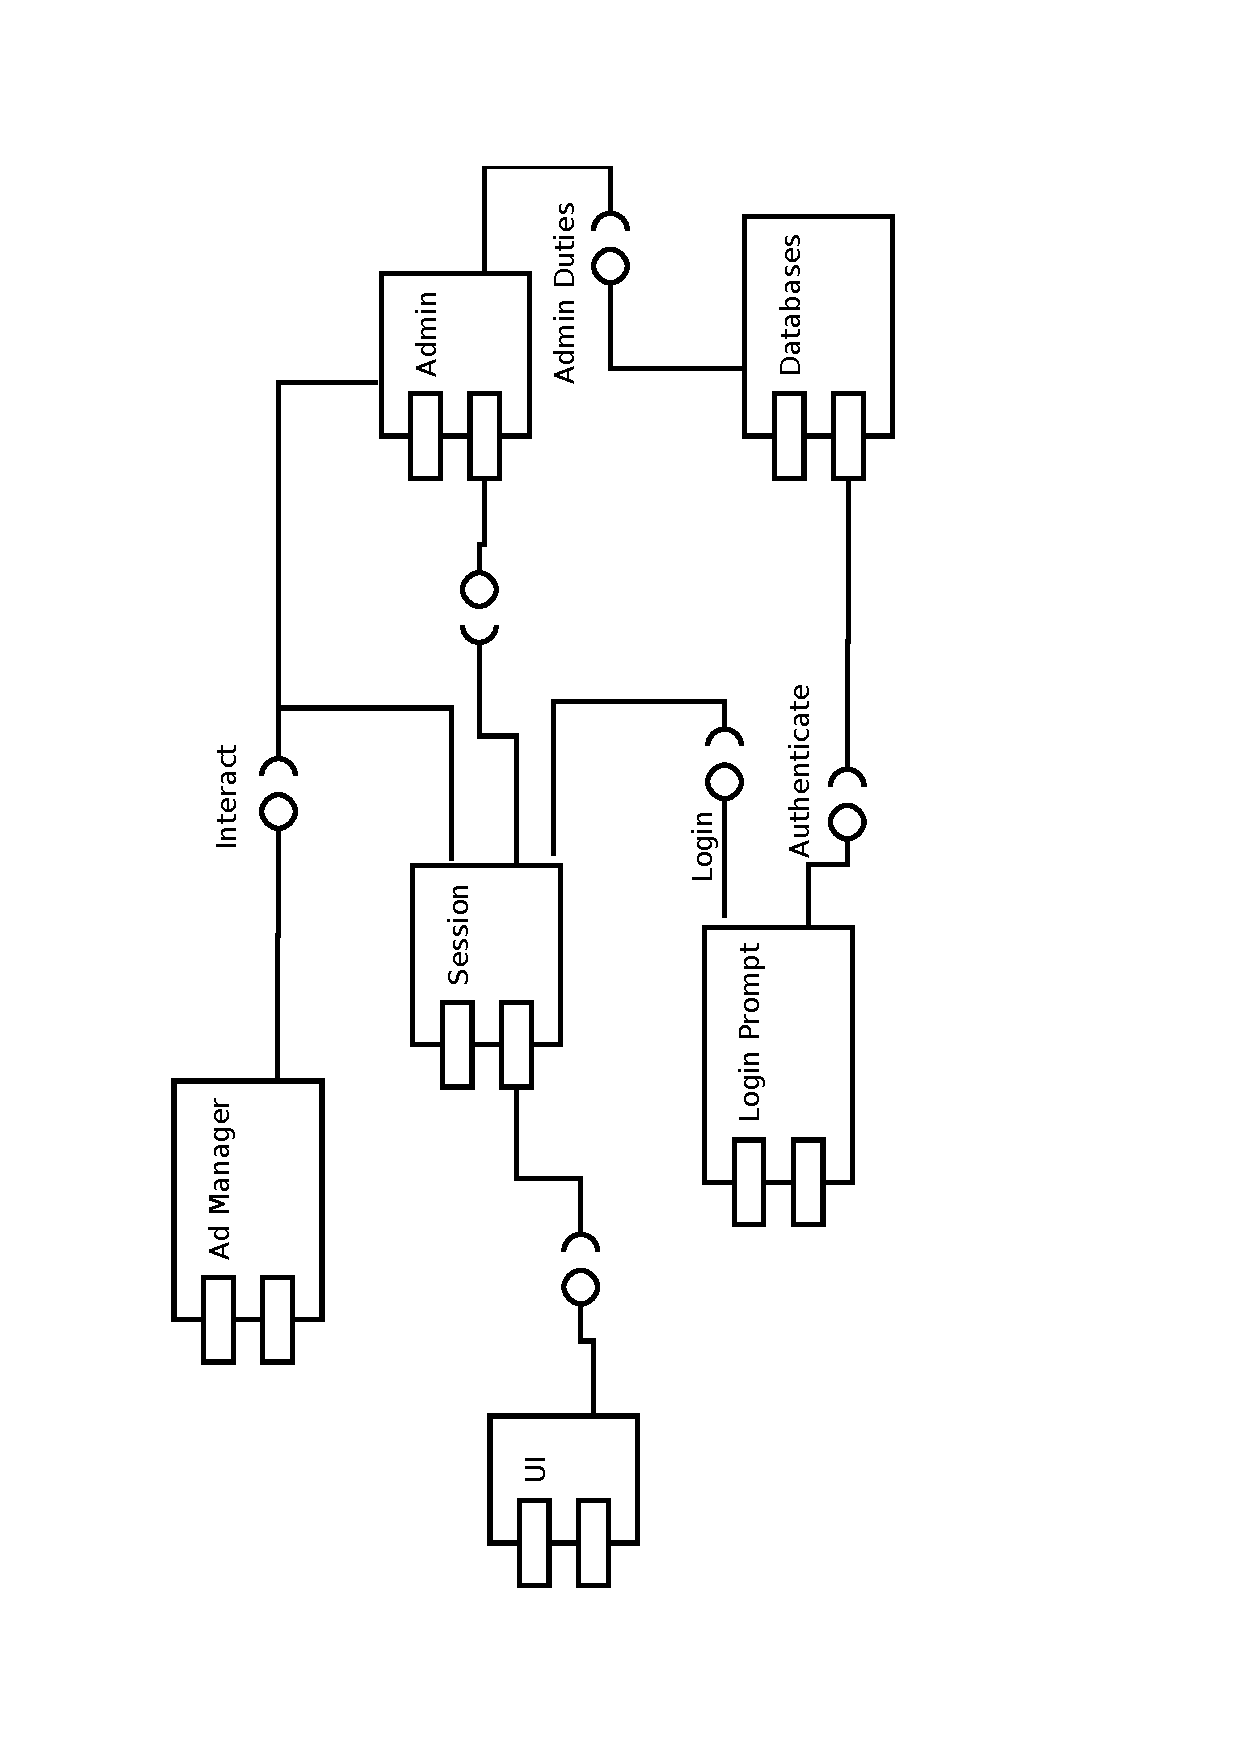
\includegraphics[width=\textwidth]{PSDDiagram.pdf}

\subsection{Rationale}

\newpage

\section{State Chart}

\newpage

\section{Class Diagrams and API Specifications}

\subsection{Advert Manager}

\subsubsection{Class Diagram}

\subsubsection{API Specification}

\subsection{Session}

\subsubsection{Class Diagram}

\subsubsection{API Specification}

\subsection{User Interface}

\subsubsection{Class Diagram}

\subsubsection{API Specification}

\subsection{Admin}

\subsubsection{Class Diagram}

\subsubsection{API Specification}

\subsection{Login Prompt}

\subsubsection{Class Diagram}

\subsubsection{API Specification}

\subsection{Database}

\subsubsection{Class Diagram}

\subsubsection{API Specification}

\textbf{Full name:} public abstract interface UserDatabase\\

\textbf{Package:} uk.ac.glasgow.internman.users

This is the interface for the user database. This database will hold information
on students, companies, and the course coordinator. For University students and
staff members, the database will access the MyCampus GUID system for login. For
companies, a separate store for their user information will be used.\\

\textbf{Methods}

\begin{itemize}

\item{\textbf{public boolean addCompany(String name, String email, String 
password)}

Add information about a company to the database.

\textbf{Preconditions:} Database must not already contain details of the 
company.

\textbf{Invariants:}

\textbf{Postconditions:} Database now contains information about a company 
including their login password.}

\item{\textbf{public Company getCompany(String name)}

Gets information about the company with the given name.

\textbf{Preconditions:}

\textbf{Invariants:}

\textbf{Postconditions:} If a valid name is given, the object associated with
the company is returned, otherwise null is returned.}

\item{\textbf{public Student getStudent(String guid)}

Gets information about the student with the given GUID from MyCampus and the
application's user specific information database (such as internship progress).

\textbf{Preconditions:}

\textbf{Invariants:}

\textbf{Postconditions:} If a valid GUID is given, the object associated with
the student is returned, otherwise null is returned. If this is the first time
a student has been asked for, a record will be added to the user specific
information database.}

\item{\textbf{public void updateStudent(Student student)}

Updates the user specific data for the supplied student. For example, when a
student obtains an internship, or has had their internship assessed.

\textbf{Preconditions:} Student must be a valid Computing Science student and
is known to the application's user database.

\textbf{Invariants:}

\textbf{Postconditions:} Student's user specific information is up to date.}

\end{itemize}

\newpage

\section{Acceptance Test Plan}

\end{document}